\documentclass[byrevtex,amssymb,aps,pra,floatfix,letterpaper]{revtex4}
\usepackage{graphicx}
\usepackage{hyperref}
\bibliographystyle{apsrev}
\date{\today}
\pagestyle{plain}
\newcommand{\degree}[0]{$^\circ$}

\begin{document}

\title{Experiment 6: Vapor pressure of a pure liquid}

\date{\today}

\maketitle

\section{Introduction}
Vapor pressure is an intensive property of a given substance, which means that the vapor pressure is independent on the amount of substance. It depends strongly on temperature, with higher temperatures resulting in increased vapor pressure. For example, if you heat liquid in a closed container, the vapor pressure keeps increasing (until the container breaks). The vapor pressure also determines the boiling point of a liquid at a given external pressure. Recall that a liquid boils when its vapor pressure becomes equal to the external pressure. Under ambient conditions the external pressure corresponds to $1.013\times 10^5$ Pa (760 torr) and the boiling point in this case is called the \textit{standard boiling point}. If the pressure is reduced, the boiling point decreases accordingly. For example, vacuum distillation is based on this principle.

In this experiment the vapor pressure of a pure liquid is measured at several temperatures and the enthalpy of vaporization is calculated using the Clausius-Clapeyron equation \cite{SILBEY,ATKINS1,TNOTES}. The enthalpy of vaporization can be used, for example, for calculating the change in boiling point when a small amount of impurities are  present \cite{ATKINS1,TNOTES}.

\section{Theory}
The Clausius-Clapeyron is based on the assumptions that the gas phase (i.e., the vapor) follows the ideal gas law and the molar volume of the liquid is negligible compared to the gas. The differential form of the equation is \cite{SILBEY,ATKINS1,TNOTES}:

\begin{equation}
\label{eq1}
\frac{dP}{dT} = \frac{P\Delta_{vap}\bar{H}}{RT^2}
\end{equation}

\noindent
where $P$ is the liquid vapor pressure (Pa), $T$ is the temperature (K), $\Delta_{vap}\bar{H}$ is the enthalpy of vaporization (J mol$^{-1}$; the over bar signifies that this is a per mole quantity), and $R$ is the molar gas constant (8.31451 J mol$^{-1}$ K$^{-1}$). Note that in Eq. (\ref{eq1}), $P$ and $T$ follow the phase boundary line in the phase diagram of the substance. By assuming that $\Delta_{vap}\bar{H}$ is temperature independent, Eq. (\ref{eq1}) can be separated and integrated (without limits):

\begin{equation}
\label{eq2}
\underbrace{ln(P)}_{y} = \underbrace{-\frac{\Delta_{vap}\bar{H}}{R}}_{k}\times\underbrace{~~\frac{1}{T}~~}_{x} 
+ \underbrace{~~~C~~~}_{b}
\end{equation}

\noindent
where $C$ is a constant of integration. If experimental values for vapor pressure $P$ and temperature $T$ are available, a plot of $ln(P)$ vs. $1/T$ should yield a straight line ($y = kx + b$) where the slope gives an estimate for the enthalpy of vaporization. The value of $\Delta_{vap}\bar{H}$ obtained from Eq. (\ref{eq2}) is an average value over the given temperature range. Note that when $\Delta_{vap}\bar{H}$ depends strongly on temperature, Eq. (\ref{eq2}) will give unreliable results. In this case the following form has been found useful in practice:

\begin{equation}
\label{eq3}
\Delta_{vap}\bar{H} = a + bT
\end{equation}

\noindent
where $a$ (J mol$^{-1}$) and $b$ (J K$^{-1}$ mol$^{-1}$) are constants. Inserting this equation into Eq. (\ref{eq1}) and integrating both sides yields a more reliable equation for determining $\Delta_{vap}\bar{H}(T)$ (Rankine-Kirchoff-Dupre equation). In this experiment it is sufficient to use Eq. (\ref{eq2}).

At constant pressure the molar entropy of vaporization $\Delta_{vap}\bar{S}$ (J K$^{-1}$ mol$^{-1}$) can be obtained from $\Delta_{vap}\bar{H}$ by the following relation \cite{TNOTES}:

\begin{equation}
\label{eq4}
\Delta_{vap}\bar{S} = \frac{\Delta_{vap}\bar{H}}{T}
\end{equation}

\noindent
where $T$ is the boiling point temperature. The Trouton's rule predicts that $\Delta_{vap}\bar{S}$ should be constant (\textit{ca}. 85 J K$^{-1}$ mol$^{-1}$) for non-associated liquids at their standard boiling points \cite{ATKINS1, TNOTES}. For example, the following values for $\Delta_{vap}\bar{S}$ have been determined 
experimentally: cyclohexane (85.1 J K$^{-1}$ mol$^{-1}$), benzene (87.2 J K$^{-1}$ mol$^{-1}$) and CCl$_4$  (85.8 J K$^{-1}$ mol$^{-1}$) \cite{TNOTES}.

\section{Measurement setup}
A schematic diagram of the apparatus is shown in Fig. \ref{fig1}. The apparatus is connected to a glass-vacuum line so that it can be evacuated. \textbf{Note that glass part break easily --- be very careful and do not use too much force!}

\begin{figure}[!htp]
\begin{center}
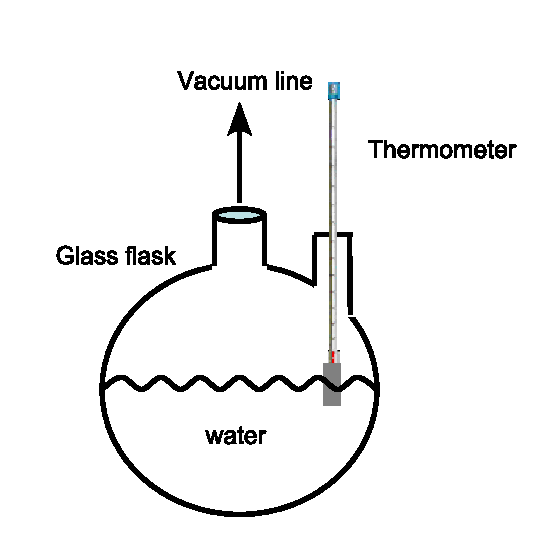
\includegraphics[scale=0.5]{fig1}
\caption{A schematic view of the vapor pressure apparatus (heater not shown).}
\label{fig1}
\end{center}
\end{figure}

\begin{figure}[!htp]
\begin{center}
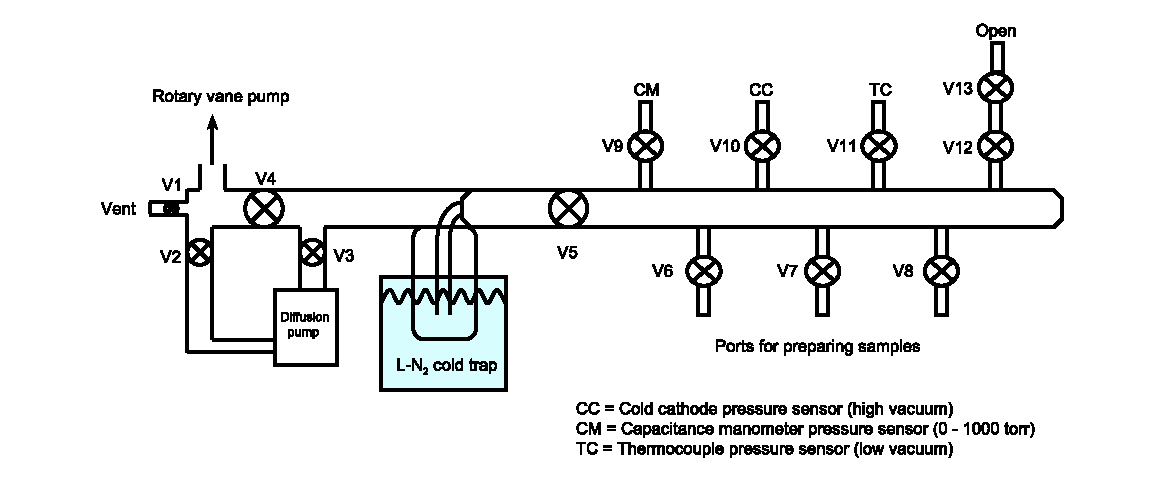
\includegraphics[scale=0.6]{fig2}
\caption{A schematic view of the vacuum line.}
\label{fig2}
\end{center}
\end{figure}

\section{Sample preparation and measurement}

In this experiment the vapor pressure of water will be determined at different temperatures. This means that you are effectively following the liquid -- gas phase
boundary line in the water phase diagram. The outcome of the experiment consists of pressure values (Pa) at each sample temperature (K).\\

\noindent
\underline{1. Installation.} Install a 500 mL three-neck round bottom flask on a heat jacket (must be at room temperature) and fix them to the metal frame holding the vacuum line. The flask should be under the sample port with valve V6 (see Figs. \ref{fig1} and \ref{fig2}). Make sure that the installation is rigid and nothing can fall off. Remember that glass parts are very fragile! Connect the middle neck of the flask to the vacuum line by using a glass tube with a ground joint (use a small amount of vacuum grease), a short flex tube, and two UltraTorr connectors. Make sure that the supporting metal tubes are installed inside the flex tube before tightening the UltraTorr. Install the fan that cools down the flex tube and prevents migration of the liquid into the vacuum line. Insert a thermometer ($\approx$ 1\degree C accuracy, minimum temperature 20\degree C, maximum temperature 110\degree C) through one of the side necks in the flask by using a vacuum feedthrough as shown in Fig. \ref{fig1} and tighten the feedthrough. Block the open neck on the other side with a glass stopper. Use a small amount of vacuum grease to make the connections vacuum  tight (i.e., the O-rings and ground glass joints). Install additional support for the thermometer, if necessary.\\

\noindent
\underline{2. Leak testing.} Make sure that all the valves (i.e., V1 -- V13) are closed. Do not use excess force when closing the valves and do not open them too far. Make sure that the Cold Cathode (CC) controller is off and that the capacitance manometer (CM) and thermocouple (TC) controllers are on. Note that the readout unit in both controllers is torr. Make sure that the rotary vane pump (on the floor; the diffusion pump is not needed in this experiment and should be off) is running. Open valves V9 and V11. This allows CM and TC to measure the pressure in the vacuum line. Open valve V6 to connect the sample flask to the vacuum line. Next open valve V4 and then slowly valve V5. Observe the reading on both controllers. The pressure should start decreasing rapidly. If no pressure drop is observed, the vacuum line is leaking and the vacuum line must be inspected for leaks (e.g., O-rings, ground joints, etc.). A more sensitive test for leaks can be made by closing valve V5 and making sure that no appreciable pressure increase is observed on the CM and TC controllers. Leave the valves V4 and V5 open and close both V6 and V11.\\

\noindent
\underline{3. Liquid nitrogen trap.} To protect the mechanical pump from excessive amounts of water, install the L-N$_2$ trap (see Fig. \ref{fig2}) by filling a Dewar flask with L-N$_2$ and securing it under the trap tube. Keep the Dewar flask filled with L-N$_2$ during the experiment.\\

\noindent
\textbf{WARNING: Use a faceshield when operating the vacuum line or the L-N$_2$ Dewar flask! Under some rare circumstances glass L-N$_2$ Dewar flasks may break and shoot pieces of glass above the flask. When handling L-N$_2$ (77 K), use wool gloves to avoid cold burns.}\\

\noindent
\underline{4. Sample preparation.} Make sure V6 is closed and remove the glass stopper from the three-neck flask. You may have to use some force in removing it since there is still vacuum inside the flask. Add about 200 mL of deionized water through the neck into the flask and block the neck again with the glass stopper. Note that the thermometer should be exposed to both the gas and the liquid (see Fig. \ref{fig1}). Open valve V6 slowly. Pump on the flask for about 20 seconds for the pressure to stabilize around 20 torr. If the pressure does not drop, close valve V6 and inspect for leaks (see above). Finally close valve V5.\\

\noindent
\underline{5. Measurements.} \textbf{If you observe liquid in the vacuum line at any point during the experiment, turn off the heater and  notify the instructor!} At each pressure, record the boiling temperature of water inside the flask. The first point should be taken around 20 torr. You should increase the temperature  (by increasing the voltage on the Variac; do not exceed 40\% of maximum voltage) until you observe that the liquid boils. Note that there is a considerable delay between increasing the voltage and actual heating. At this point, you should record the temperature from the thermometer. This gives the  first ($P$, $T$) point. Pressure inside the vacuum line can be increased  by the following procedure (by about 10 torr): open V13, close V13, open V12 and close V12. If a higher pressure increase is desired, this procedure can be repeated many times or V12 can be opened slightly while keeping V13 open. The latter procedure is tricky as it is difficult to control the amount of air entering the vacuum line whereas the former method is, on the other hand, rather slow because it must be repeated many times. If too much air enters the vacuum line, you must pump the excess air out of the line by opening V5 slightly and finally leaving it closed. Carry out your measurements at 10 different pressures distributed between 20 and 600 torr. Each time you increase the voltage on the Variac, be sure to wait for the temperature to stabilize. \textbf{Do not exceed 100\degree C temperature.}\\

\noindent
\underline{6. Finishing up.} Make sure that all valves (i.e., V1 -- V13) are closed. Turn off the heat jacket and let it cool down. Remove the heat jacket and disconnect the flex tube from the vacuum line so that the three-neck flask can be removed. Watch out for the thermometer! Detach the parts from the flask. Empty the vacuum line by opening valves V4 and V5 slowly. After the line has pumped down, close V4, remove the L-N$_2$ Dewar flask and let air into the vacuum line by slowly opening V7 (leave it open). At this point, the excess water from the vacuum line has condensed in the trap. Carefully detach the trap tube from the vacuum line. Leave the trap in a hood so that water can evaporate or, alternatively, you may clean the tube. The trap tube should be installed back into the vacuum line after water has been removed. Finally, open V5 slowly to evacuate the vacuum line again. Leave the rotary vane pump on.

\section{Data analysis}

Analyze your data using the qtiplot program (see the general section of the laboratory manual; qtiplot). Enter your temperature (X) and pressure (Y) data into an empty table in SI units. After you have entered the values, transform your variables to $1/T$ (X-axis) and $\ln(P)$ (Y-axis). For the X axis, select the X column by clicking on the column header with mouse, choose ``Table $\rightarrow$ Set Column Values...'' and enter the following expression in the large input box: 1/col("1") and click on Apply and Close. For the Y axis, select the Y column by clicking on the column header with mouse, choose ``Table $\rightarrow$ Set Column Values...'' and enter the following expression in the large input box: ln(col("2")) and click on Apply and Close. Finally choose ``Analysis $\rightarrow$ Fit Linear'' from the top menus to fit a straight line to your data. According to Eq. (\ref{eq2}) the slope gives the vaporization enthalpy (J mol$^{-1}$) along with its error estimate. Include the graph, which shows the fit between your experimental and the Clausius-Clapeyron equation, in your laboratory report. If you are not satisfied with the quality of the fit, you may also try the Rankine-Kirchoff-Dupre equation.

\section{Written laboratory report}

\noindent
Follow the general instructions for written laboratory reports and for the results section include:\\

\noindent
\textit{Results.} This section should include the graphs prepared above. Provide your values for $\Delta_{vap}\bar{H}$ and $\Delta_{vap}\bar{S}$ (see Eqs. (\ref{eq2}) and (\ref{eq4})) along with the error estimates. Try to assess the linearity (or non-linearity) of the graphs. If your data shows observable non-linearity, try to explain the why this is so. Provide also experimentally observed reference values for $\Delta_{vap}\bar{H}$ and $\Delta_{vap}\bar{S}$ (see, for example, Ref. \cite{ATKINS1}).

\section{References}

\vspace{-1cm}

\bibliography{../../references}

\end{document}
